\documentclass{beamer}

\usepackage[frenchb]{babel}
\usepackage[T1]{fontenc}
\usepackage[utf8]{inputenc}

\usetheme{Warsaw}

\usepackage{amsmath}
\usepackage{amssymb}
\usepackage{amsthm}
\usepackage{hyperref}
\usepackage{graphicx}
\usepackage[space]{grffile}

\usepackage{listings}
\lstset{language=Java}

\newcommand{\class}[1]{\texttt{#1}}

\title[Big data sampling and applications]{Big data sampling\\Shakespeare, web and networks\\Project defense}
\author{Gaspard FEREY \& Jonathan VISBECQ}
\institute{Bruno SALVY\\perso.ens-lyon.fr/bruno.salvy/INF431/Projet}
\date{June 18, 2012}


\AtBeginSection[]
{
\begin{frame}
  \tableofcontents[currentsection, hideothersubsections]
\end{frame}
}



\begin{document}

\logo{
\includegraphics[height=50pt]{pictures/logoX.png}}

\begin{frame}
\titlepage
\end{frame}

\begin{frame}
  \frametitle{Contents}
  \tableofcontents[hideallsubsections]
\end{frame}


\section{Hash functions}

\subsection{Superclass}
\begin{frame}[fragile]
\frametitle{Hash functions}
\framesubtitle{The abstract superclass}

\begin{block}{The HashFunction superclass}
\begin{verbatim}
 public abstract class HashFunction {
     public int hashByteArray(byte[] array);
     public int hashString(String s);
 }
\end{verbatim}
\end{block}

\end{frame}


\subsection{Main functions}
\begin{frame}
\frametitle{Main functions}
\begin{itemize}
\item LookUp3
\item MurmurHash3
\item DJB2
\item JavaHash
\item LoseLose
\item HomemadeHash
\end{itemize}
\end{frame}

\subsection{Tests}
\begin{frame}
\frametitle{Tests}

Insérer le tableau ici

\end{frame}



\section{The HyperLogLog Algorithm}

\subsection{The algorithm}
\begin{frame}
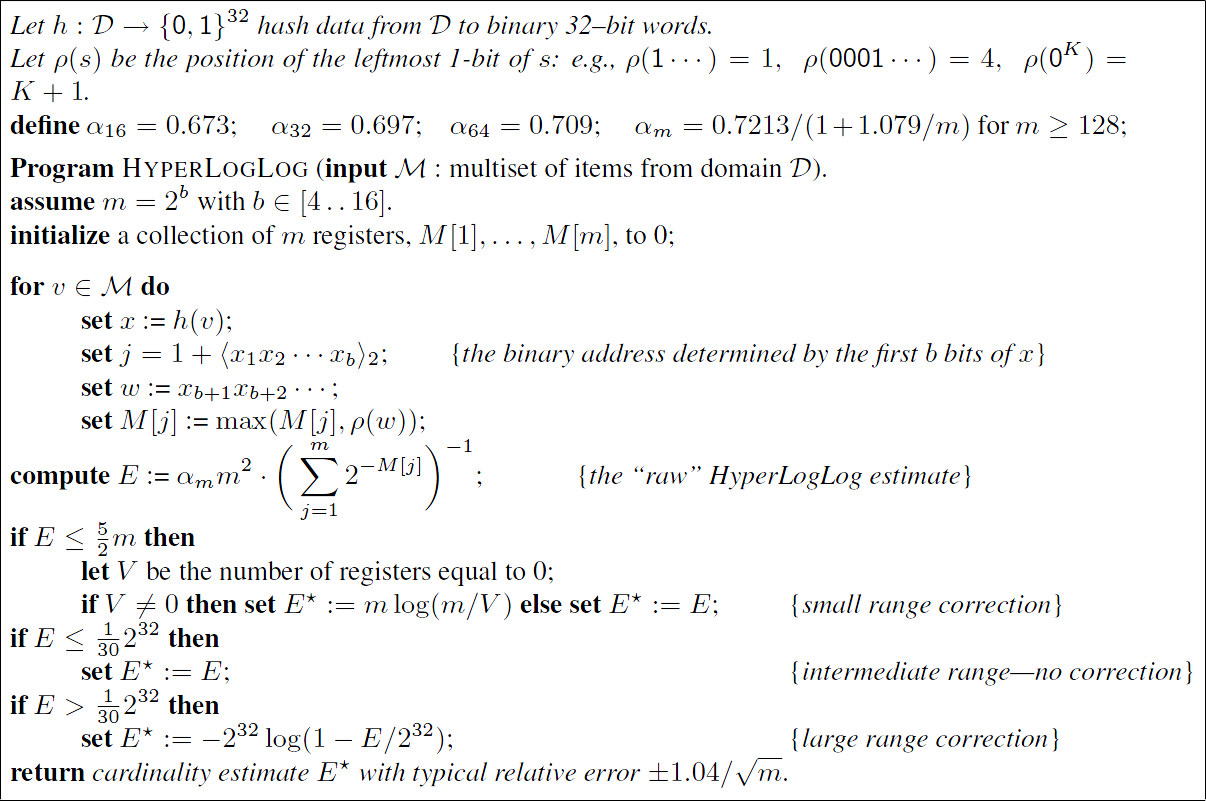
\includegraphics[scale=0.3]{pictures/algoFlajolet.png}
\end{frame}

\begin{frame}[fragile]

\begin{block}{The $\alpha$ tab}
\begin{verbatim}
static double[] alpha = {0 , 0.351194 , 0.532435
        , 0.625609 , ... };
\end{verbatim}
$\texttt{alpha[b]} = \alpha_m$ where $m = 2^b$.\\
Value computed with Wolfram Mathematica
\end{block}

\begin{block}{The $\rho$ function}
\begin{verbatim}
  public static int rho ( long x )
\end{verbatim}

\end{block}
\end{frame}


\begin{frame}[fragile]
\begin{block}{Building the $M$ collection}
\begin{verbatim}
public static int[] buildFingerPrint (Path path,
          HashFunction func , int b , int k )
\end{verbatim}

\end{block}

\begin{block}{Handling the $k$-shingles}
To read a new word
\begin{verbatim}
strBuilder.append( s );
indexes.add( s.length() );
\end{verbatim}
To remove the last word
\begin{verbatim}
strBuilder.replace( 0, indexes.poll(), "");
\end{verbatim}
\end{block}

\end{frame}



\subsection{Similarities}
\begin{frame}
Empty frame
\end{frame}



\section{Sliding windows}

\subsection{The algorithm}
\begin{frame}
\textbf{assume} $m = 2^b$ with $b\in[4...16]$.\\
\textbf{initialize} a collection of $m$ lists M[1], ..., M[m] to empty\\


\end{frame}

\subsection{Complexity}
\begin{frame}
Empty frame
\end{frame}




\section{Significant words}

\subsection{Significant word sample}
\begin{frame}
Empty frame
\end{frame}

\subsection{Complexity}
\begin{frame}
Empty frame
\end{frame}

\subsection{Mice}
\begin{frame}
Empty frame
\end{frame}


\section{Icebergs}

\begin{frame}
Empty frame
\end{frame}



\section*{Conclusion}

\begin{frame}
\title{Conclusion}
Empty frame

\end{frame}

 
\end{document}
